%!TEX encoding = UTF-8 Unicode
% !TeX spellcheck = en_GB
%%%%%%%%%%%%%%%%%%%%%%%%%%%%%%%%%%%%%%
\chapter{Constraints on the Higgs properties }\label{chap:HiggsConstr}
%%%%%%%%%%%%%%%%%%%%%%%%%%%%%%%%%%%%%%
In this chapter, I will discuss some of the bounds on the Higgs sector . Starting from an overview of the theoretical constraints on the Higgs potential, like the quantum triviality and unitarity. Then, the state-of-the-art experimental results on Higgs properties and couplings measurements will be discussed. However, despite many of the Higgs boson properties have been measured with good accuracy, there are still difficult observables in the Higgs sector and some open problems. These will be addressed at the end of this chapter.   
%%
\section{Theoretical constraints}
 \subsection{Electroweak precision data fits }
Even prior to the discovery of the Higgs boson at LHC in 2012, many theoretical aspects of the Higgs sector provided marked bounds on the Higgs properties, particularly it mass. For instance, using the EWPO measurements at LEP provided an input for a fit based of radiative effects coming from the Higgs boson to such observables ~\cite{ALEPH:2005ab} as in diagram (a) of ~\autoref{fig:ewdiagrams}, the bounds improved with the improvements of EWPO measurements, these bounds were known as the `` blue band'' plots seen with their progression in~\autoref{fig:buleband}.
  \begin{figure}[b!]
  	\begin{center}
  		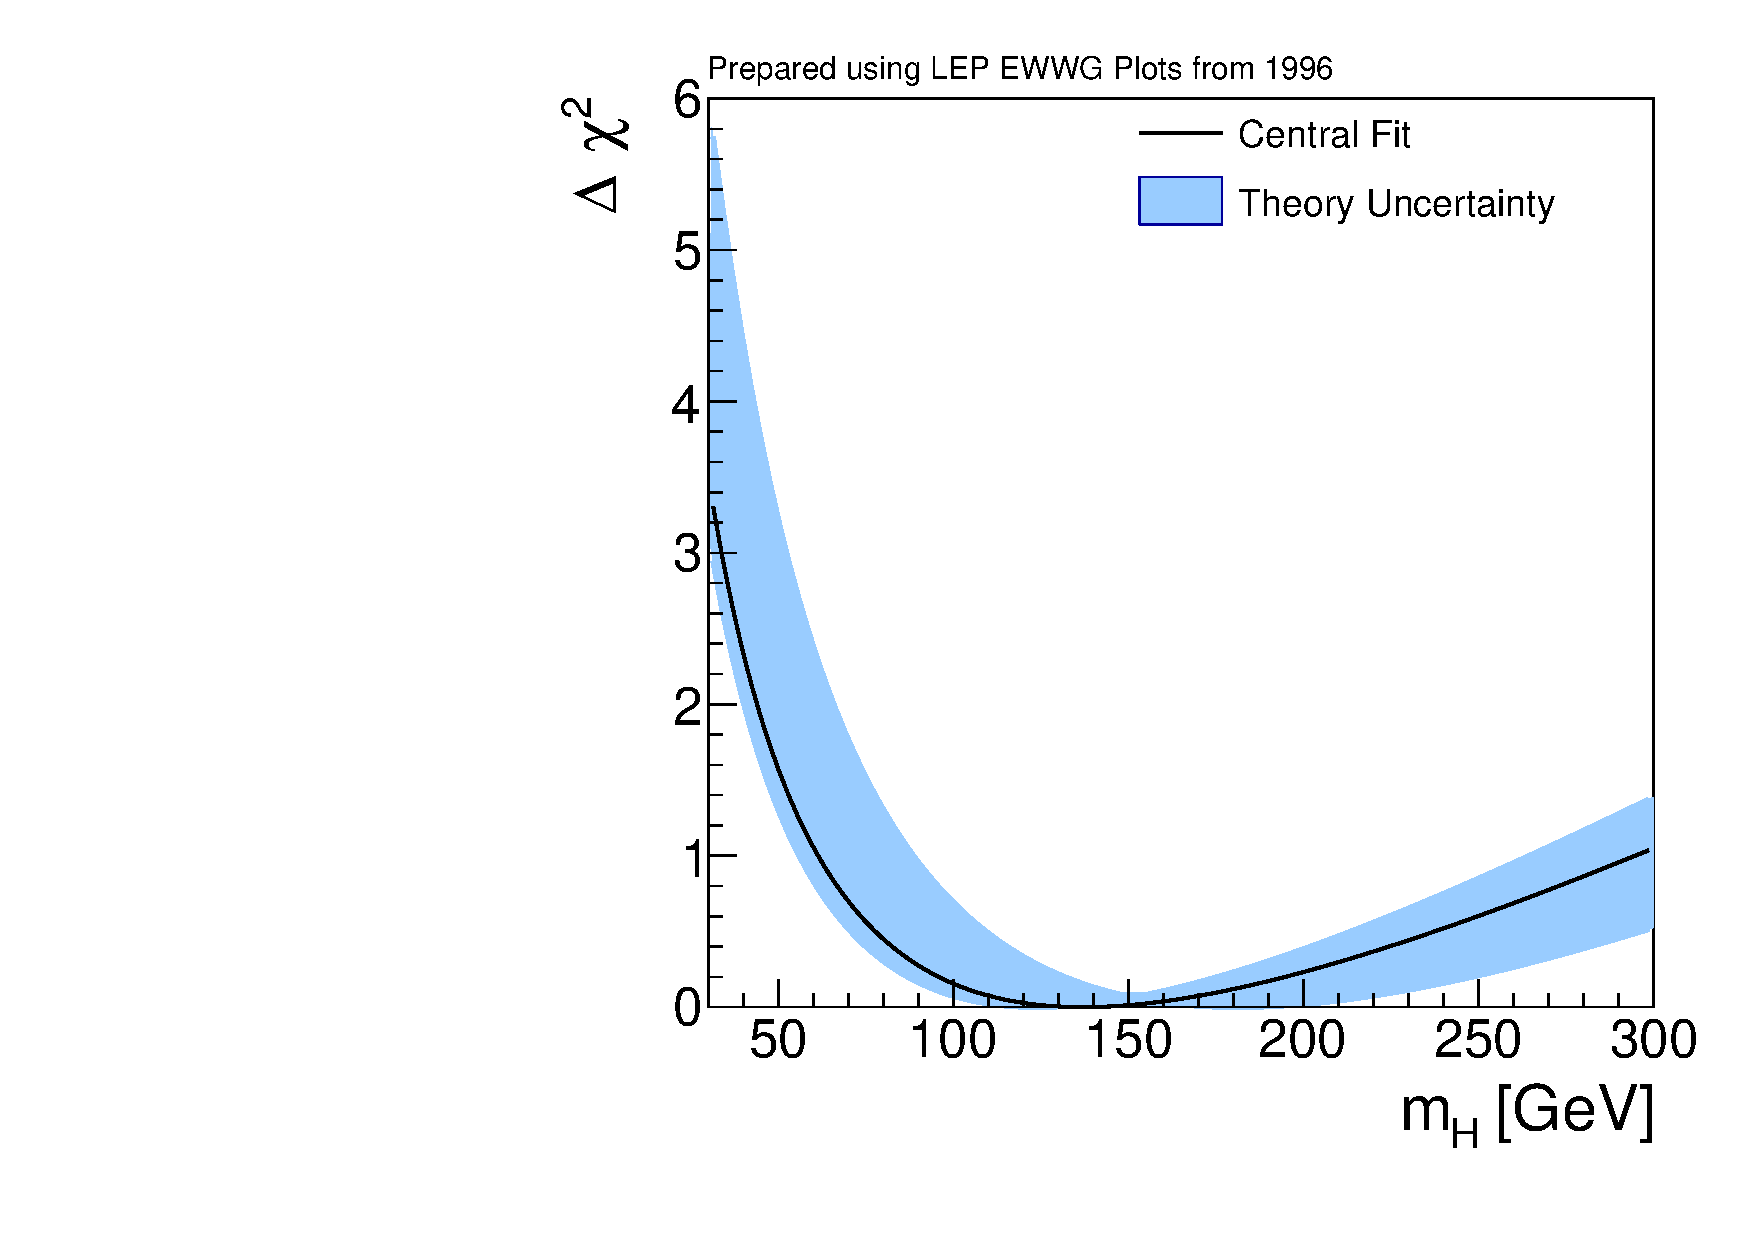
\includegraphics[width=.275 \linewidth]{figures/blueband/BlueBand_1996}
  		\hspace{-0.75 cm}
  		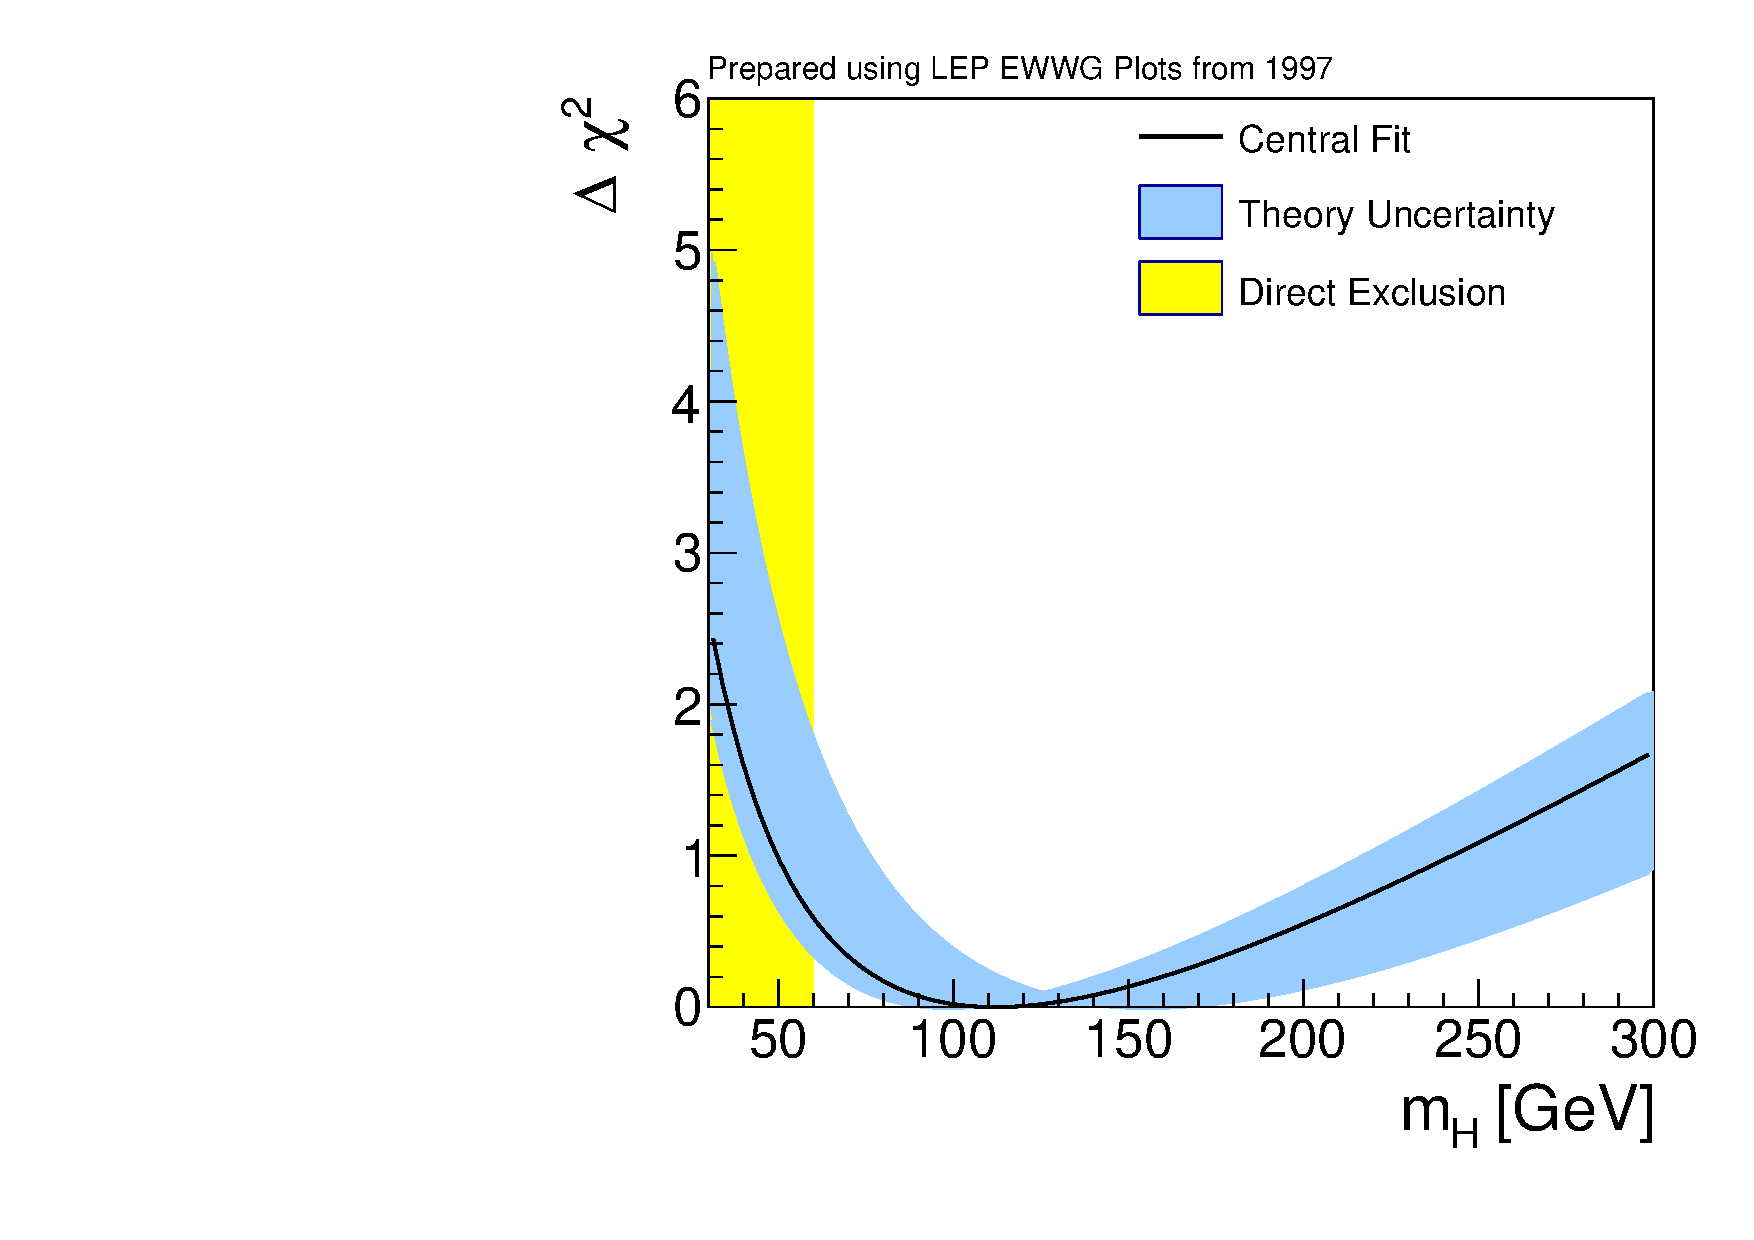
\includegraphics[width=.275 \linewidth]{figures/blueband/BlueBand_1997}
  			\hspace{-0.75 cm}
  		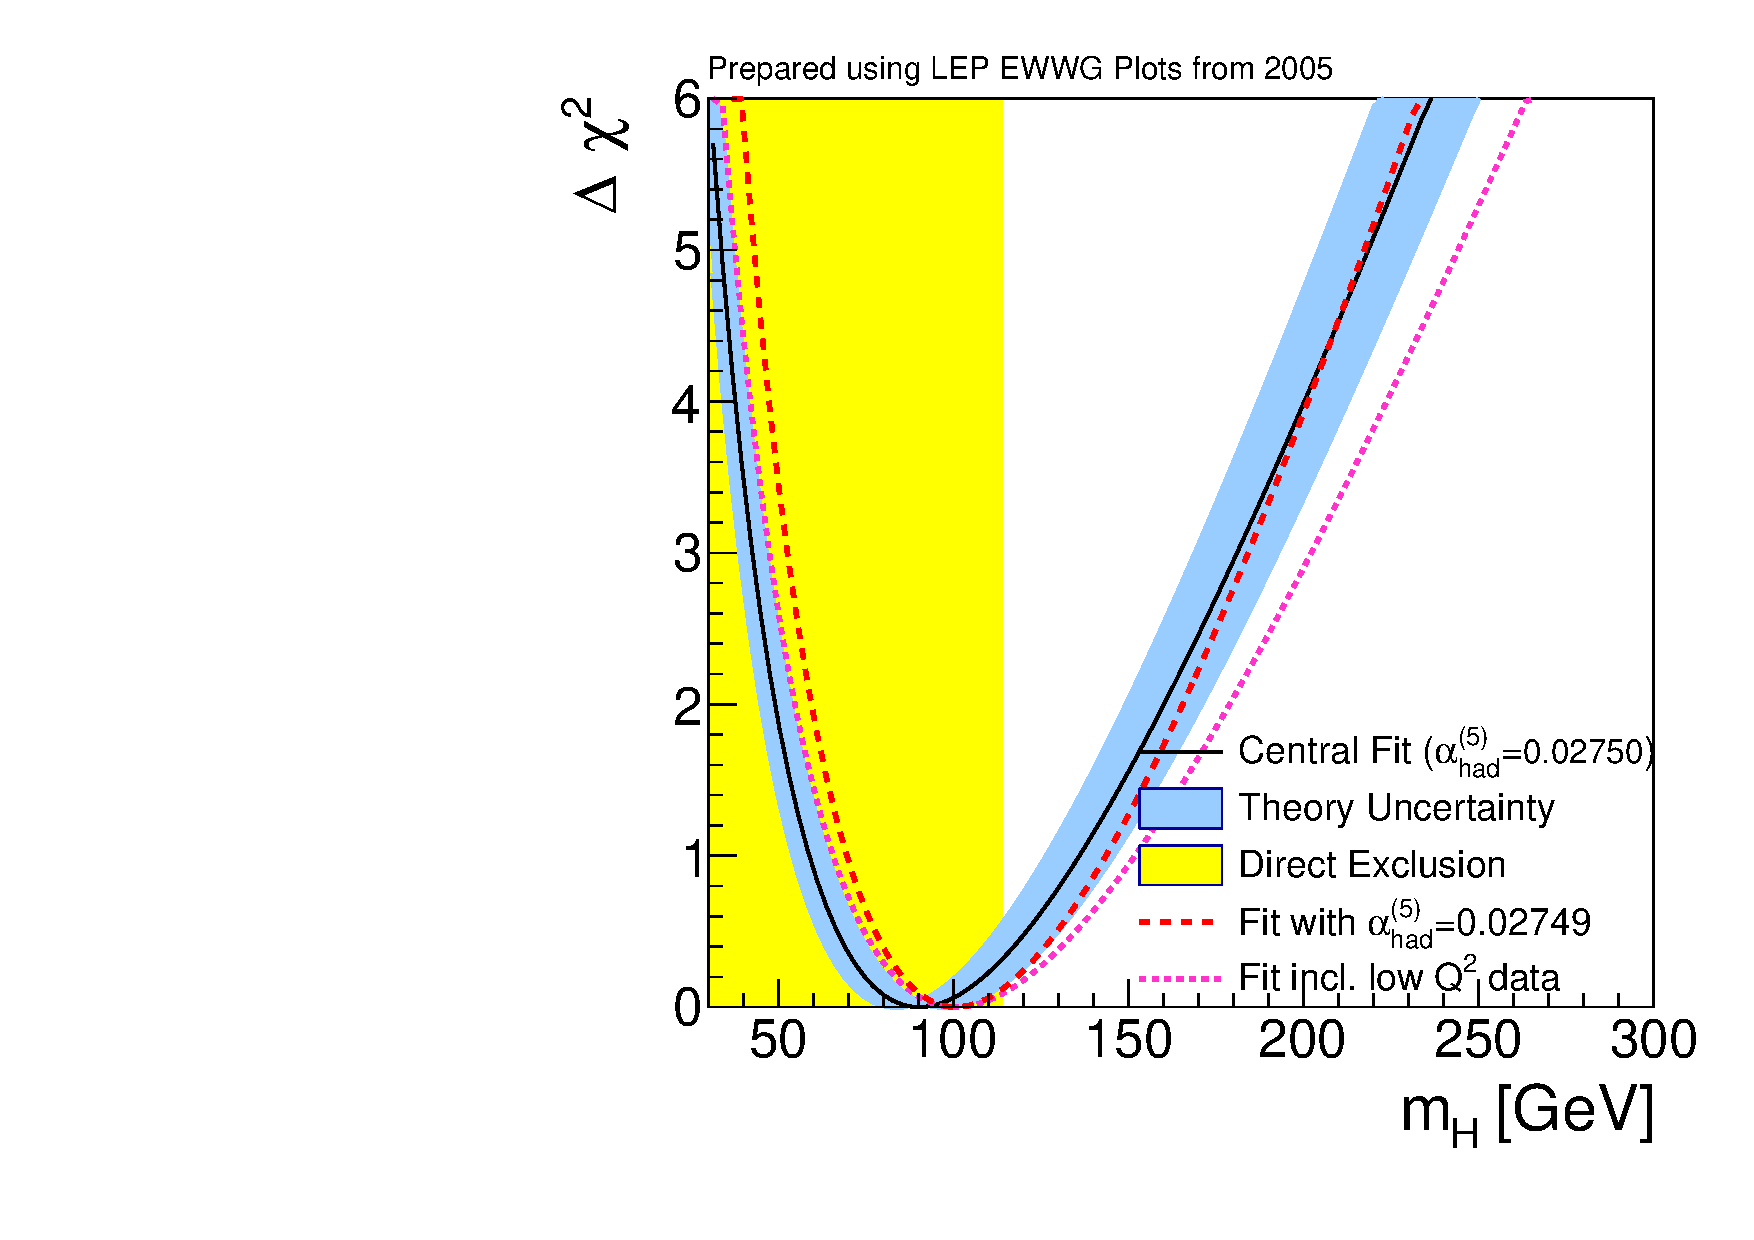
\includegraphics[width=.275 \linewidth]{figures/blueband/BlueBand_2005}
  			\hspace{-0.75 cm}
  			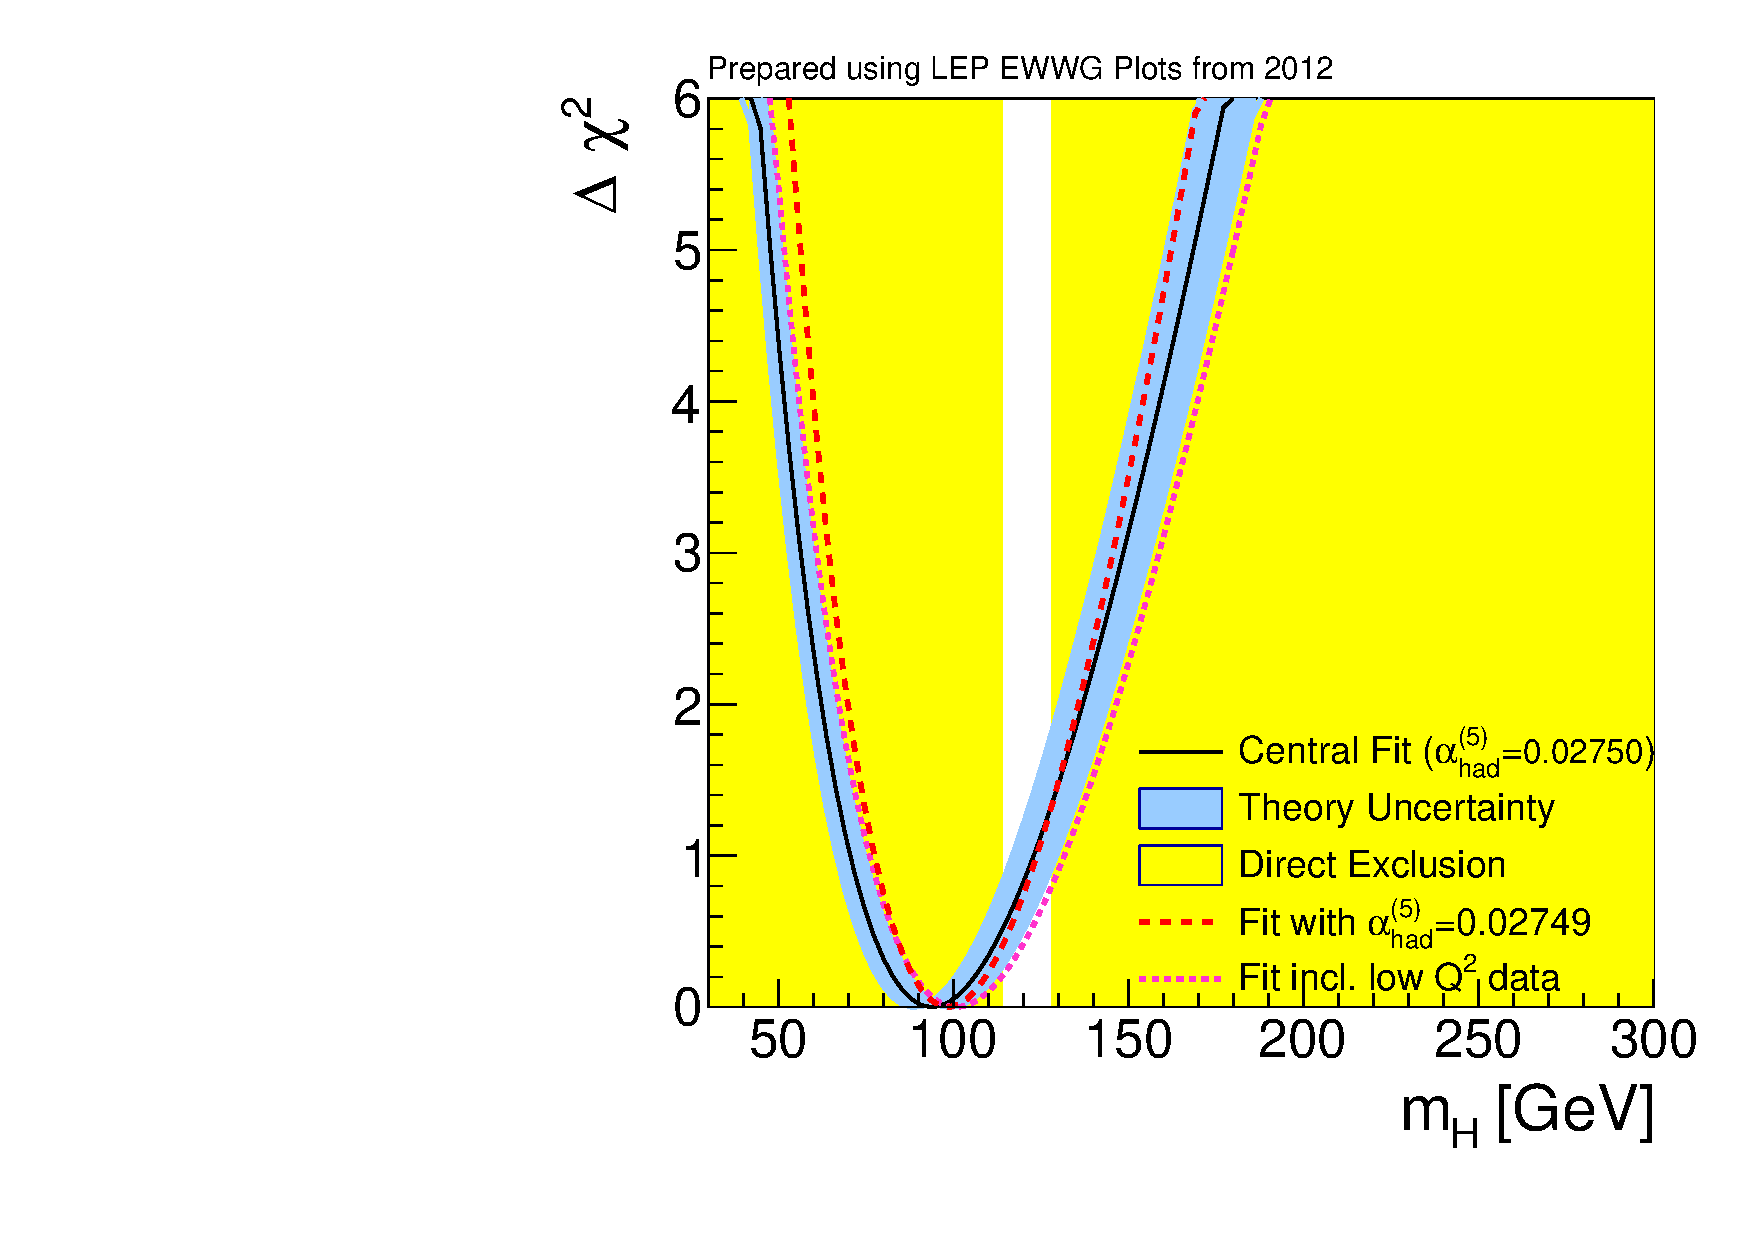
\includegraphics[width=.275 \linewidth]{figures/blueband/BlueBand_2012}
  		\caption{Progression of the ``blue band'' plots with LEP data from 1996 up to 2021 prior to the announcement of the Higgs boson discovery. There plots were taken from~\cite{Erler:2019hds}, based data from LEP~\cite{ALEPH:2005ab} \label{fig:buleband} }
  	\end{center}
  \end{figure}
  \begin{figure}[t!]
	\begin{center}
		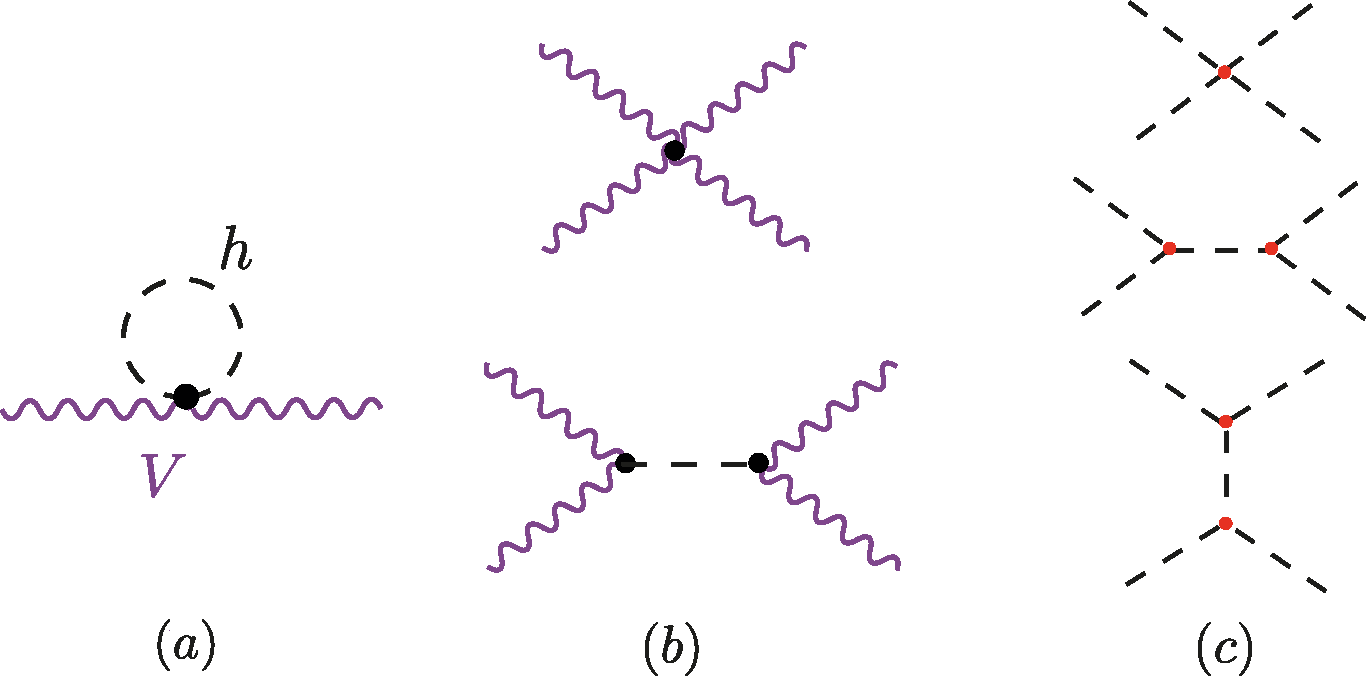
\includegraphics[width=.7 \linewidth]{figures/theoretical_const}
		\caption{Diagrams contributing to theoretical bounds on the Higgs, $(a) $ shows an example of radiative corrections to EWPO from the Higgs bosons. The diagrams in $(b)$ show an elastic scattering of EW vector bosons leading to a bound on the Higgs mass from perturbative unitarity, similarly in $(c)$ diagrams for $hh \to hh$ scattering leading to constraints on Higgs self-coupling.}
		\label{fig:ewdiagrams}
	\end{center}
\end{figure}
 \subsection{Partial-wave unitarity}. This process
 Another bound on Higgs mass emerged from studying the amplitudes of EW vector bosons elastic scattering having longitudinal polarisations $V_L V_L \to V_L V_L$ at high energies~$ E \gg m_W$ (see diagrams (b) in~\autoref{fig:ewdiagrams} ), where the Goldstone equivalence theorem holds ~\cite{PhysRevD.42.853}. 
 This bound comes from applying the partial wave perturbative unitarity on the EW boson scattering amplitude. I will derive here this bound starting from the \textbf{Optical theorem}, which a direct result from the unitarity of the $\mathbf S$ matrix.
 \begin{tcolorbox}[title=The optical theorem,
 	title filled=false,
 	colback=Mahogany!5!white,
 	colframe=Mahogany]
 	Let $\mathcal M_{aa}$ be a covariant matrix element for an elastic  scattering process with for a particle $a$  then the following relation applies
\begin{equation}
	\sum_{f}  \int d\Phi_n(p_a,p_i^f)| \mathcal M_{af}|^2 = 2 \mathfrak{I}( \mathcal M_{aa}),
	\label{opt}
\end{equation}
where the sum is over all intermediate sates $n$-particle states $f$ with momenta $p_i^f$ and $d\Phi_n(p_a,p_i^f)$ is the $n$-particle phase space.
 \end{tcolorbox}
If we only consider a $2 \to 2$ process with momentum states. $\ket{p_1,p_2} \to \ket{k_1,k_2}$, then~\eqref{opt}, after expanding the $2$-particle phase space ,
 simplifies to 
\begin{align}
	&\int  \frac{d^3k_1}{(2 \pi)^3\,2E_1} \int  \frac{d^3k_2}{(2 \pi)^3\,2E_2} (2 \pi)^4 \delta^4(p_1+p_2-k_1-k_2)\,| \mathcal M (s,t)|^2 ,\nonumber \\
	&= \frac{1}{16 \pi} \int_{-1}^{1} d(\cos \theta) | \mathcal M (s,t)|^2.
\end{align}


Where $d\Phi_n(p_a,p_i^f)$ is the $n$-particle phase space, for the $2\to2$ case, the equality is substituted by $\leq$. \\ From now one, we shall only consider the $2\to2$ case  ($\ket{p_1,p_2} \to \ket{k_1,k_2}$) in which we could simplify the phase space further, rewriting the LHS of \eqref{opt} as
\begin{align}
	&\int  \frac{d^3k_1}{(2 \pi)^3\,2E_1} \int  \frac{d^3k_2}{(2 \pi)^3\,2E_2} (2 \pi)^4 \delta^4(p_1+p_2-k_1-k_2)\,| \mathcal M (s,t)|^2 ,\nonumber \\
	&= \frac{1}{16 \pi} \int_{-1}^{1} d(\cos \theta) | \mathcal M (s,t)|^2,
\end{align}
with the Mandelstam variables 
\begin{align}
          s = &k_1+k_2 \nn \\
          t =& k_1-p_1 \nn \\
          u=& k_1-p_2 \\
          s+t+&u = 4 m^2 \nn
\end{align}
Recall that the relation between the Mandelstam variable $t$, and the scattering angle for the elastic scattering is given by
\begin{equation}
	t = \frac{1}{2} (s-4 m^2)(\cos \theta-1)
\end{equation}
We could expand the matrix element $\mathcal M (s,t)$ in terms of \emph{partial waves}, isolating $s$ from scattering angle dependence
\begin{equation}
	\mathcal M (s,t) = 16 \pi \sum_j (2j+1)a_j P_j(\cos \theta).
\end{equation}
Where $a_j $ are called the $j$th partial wave amplitude, and  $P_j(\cos \theta)$ are the Legendre polynomials 
\begin{equation}
	P_j(z) = \frac{1}{j!}\frac{1}{2^j} {d^j\over dz^j} (z^2-1)^j
\end{equation}
Which satisfies the orthonormality condition
\begin{subequations}
	\begin{align}
		\int_{-1}^{1} dz \,P_j(z) P_k(z) &= \frac{1}{2j+1} \delta_{jk} \\
		P_j(1) &= 1 \,\,\, \forall j.
	\end{align}
\end{subequations}
We hence get for the LHS of \eqref{opt} scattering 
\begin{align}
	&\int  \frac{d^3k_1}{(2 \pi)^3\,2E_1} \int  \frac{d^3k_2}{(2 \pi)^3\,2E_2} (2 \pi)^4 \delta^4(p_1+p_2-k_1-k_2)\,| \mathcal M (s,t)|^2 ,\nonumber \\
	&= \frac{1}{16 \pi} \int_{-1}^{1} d(\cos \theta) \left[ 16 \pi \sum_j (2j+1) a_j(s) P_j(\cos \theta)\right] \times \nonumber\\ & \qquad \left[ 16 \pi \sum_k (2k+1) a_k^*(s) P_k(\cos \theta)\right], \nonumber \\
	&\Rightarrow \; = 32 \pi \sum_j (2j+1)| a_j(s)|^2.
\end{align}
And the RHS of \eqref{opt}
\begin{equation}
	2 \mathfrak{I}( \mathcal M_{aa}) = \underbrace{2 \mathfrak{I}( \mathcal M(s,0))}_{\color{Mahogany}\text{$t$ is integrated out.}} = 32 \pi  \sum_j (2j+1) \mathfrak{I} (a_j(s)). 
\end{equation}
Otherwise large cancellations needed, $a_j(s)$'s are hierarchal. Thus, we could compare the partial wave amplitudes term-by-term 

\begin{equation}
	| a_j(s)|^2 \leq \mathfrak{I} (a_j(s)) \;\;\; \Rightarrow \mathfrak{R} (a_j(s))^2+ \mathfrak{I} (a_j(s))^2 \leq \mathfrak{I} (a_j(s))
\end{equation}
Rearranging terms, we get
\begin{equation}
	\mathfrak{R} (a_j(s)) +\left( \mathfrak{I} (a_j(s))- \frac{1}{2} \right)^2 \leq \frac{1}{4}
\end{equation}
The partial wave amplitude has to lie within the unitarity circle. We use though perturbation theory if the  partial wave amplitude respects the inequality
\begin{equation}
	\mathfrak{R} (a_j(s)) \leq \frac{1}{2}
	\label{pwu}
\end{equation}
This is known as the perturbative partial wave unitarity bound.  \\
When~\eqref{pwu} is applied for  $V_L V_L \to V_L V_L$, in the Goldstone boson equivalence theorem regime in particular for $V=W$ boson, we get for the $S$-wave partial amplitude
\begin{equation}
a_0 \sim \frac{m_h^2}{16 \pi  v^2} \left( 2+\mathcal{O} \left(m_h^2/s \right) \right) .
\end{equation}
Looking at the asymptotic behaviour as $ s \to \infty$, we obtain the bound
\begin{equation}
	\frac{m_h^2}{8 \pi v^2} < {1\over 2}  \Leftrightarrow  m_h \leq 870 \,\GeV.
\end{equation}
Indeed this bound is obsolete now after th Higgs mass measurement, however it is very important to demonstrate the power of this technique in constraining Higgs parameters. As this method can be applied to any elastic scattering with the Higgs acts as a mediator like $ZZ\to ZZ$, $WW \to ff$ and constrain the correspong couplings $ g_{ZZh}, g_{f\bar f h}$ and so on. An important bound can be derived by examining the Higgs elastic scattering~$hh \to hh$ shown in $(c)$ of~\autoref{fig:ewdiagrams} in order to set bounds on Higgs self-interactions~$g_{hhh}$ and $g_{hhhh}$. This is what exactly has been done in ref.~\cite{DiLuzio:2017tfn}  where they have found that the $S$-wave partial amplitude for this process is given by
\beq 
\label{a0hhtohh}
a_0= - \frac{1}{2} \frac{\sqrt{s(s-4 m^2_h)}}{16 \pi s} \left[ g_{hhh}^2\left(\frac{1}{s- m_h^2} 
- 2 \frac{\log\frac{s-3m^2_h}{m^2_h}}{s-4m^2_h} \right) + g_{hhhh} \right] \, ,
\eeq
which leads to unitarity bounds on the trilinear~$g_{hhh}$ and the quartic ~$g_{hhhh}$ couplings 
\beq
\label{unitaritybounds}
\abs{g_{hhh} / g^{\rm SM}_{hhh}} \lesssim 6.5 
\qquad \text{and} \qquad
\abs{g_{hhhh} / g^{\rm SM}_{hhhh}} \lesssim 65 \, .
\eeq
A stringer constrained can be obtained by looking at the one-loop correction to the $hh\to hh$ scattering amplitude, within the full kinematic range.
% The bound on the trilinear Higgs self-coupling becomes
%\beq 
%\label{deltahhhkin}
%\Delta g_{hhh} (\sqrt{s}, m_h) = - \frac{1}{16 \pi^2} g_{hhh}^3 C_0 (m_h^2, m_h^2, s; m_h, m_h, m_h) \, ,
%\eeq 
%where $C_0$ is the scalar three-point one-loop function.
 The unitarity bound here is obtained by looking at the one-loop  amplitude at the threshold, and is given by
\beq 
\label{pertboundhhhmax}
\abs{g_{hhh} / g_{hhh}^{\text{SM}}} \lesssim 6 \, .
\eeq
These bounds are, hitherto, the strongest on these two couplings even when compared to the ones coming from current experimental searches. 
\subsection{Other bounds}
\par Further theoretical bounds could be obtained by studying quantum effects on the Higgs potential. For example, if we looked at the solution of the renormalisation group equation~(RGE) for the Higgs self-coupling~$\lambda$ with the boundary condition $ \lambda(v)=\lambda_0$ and ignoring other SM particle-contributions
\begin{equation}
  \lambda (Q^2) = \frac{\lambda_0}{1-\frac{3}{4 \pi^2} \log {Q^2\over v^2}}
  \label{eq_lambdarunnung}
\end{equation}
We see that the running of $\lambda$ will hit a pole, known as \textbf{Landau pole} when the denominator vanishes. This will happen at the scale
\begin{equation}
	Q_{{\rm c}} = v e^{4 \pi^2/3 \lambda_0} =  v e^{4 \pi^2 v^2/3 m_h^2}
\end{equation}
This indicates that the theory will break down at scales larger or equal to $ Q_{{\rm c}} $. Since the ``critical scale'' is a function of the Higgs mass, this allows us to set an upper limit on the Higgs mass assuming the SM will be valid up to a certain scale~$ Q_{{\rm c}} $. This bound is known as \textbf{quantum triviality } bound~\cite{Lindner:1985uk}. This is because the low energy behaviour of ~\eqref{eq_lambdarunnung} leads to a vanishing interaction, and if we want the Higgs Lagrangian to bee perturbative for all scales, then $\lambda$ has to be vanishing and the theory becomes non-interacting or \emph{trivial}. 
\par Another bound coming from the RGE of $\lambda$ is the \textbf{stability bound }, which considers the stability of the Higgs potential given the running of $\lambda$  by requiring that the Higgs potential is an operator bounded from below. This bound is obtained by approximating the solution of the RGE at small $\lambda$ 
\begin{equation}
\lambda(Q^2)\sim \lambda_0 +\frac{1}{16 \pi^2} \left[ - \frac{12m_t^4}{v^4} + \frac{3}{16} \left( 2g_2^4+(g_2^2+g_1^2)^2\right) \right] \log{Q^2\over v^2}
\end{equation}
For the Higgs potential to be bounded from below $\lambda(Q^2)$ ought to be $\lambda(Q^2) > 0$. With th relation for $\lambda_0$ in terms of the mass, we get a bound on $m_h$ 
\begin{equation}
m_h^2 > \frac{v^2}{8 \pi^2} \left[ - \frac{12m_t^4}{v^4} + \frac{3}{16} \left( 2g_2^4+(g_2^2+g_1^2)^2\right) \right] \log{Q^2\over v^2}
\end{equation}
Which leads to $ m_h \approx 130$\ \GeV \ if we assume that the SM is valid up to the Grand Unified Theory~(GUT) scale of $ \sim 10^{16}$ \ \GeV \ and $ m_h \approx 180$ \GeV \ for $Q$ being at the Planck scale ~$ \sim 10^{19}$ \ \GeV  . 
\par More sophisticated calculations and discussion for the Higgs potential and vacuum stability has been a subject of great interest in pre and post-Higgs discovery eras cf.~\cite{Lindner:1985uk,Sher:1988mj,Casas:1996aq,Isidori:2001bm} and the most state-of-the-art calculation for the vacuum stability at NNLO has been preformed in ref.~\cite{Degrassi:2012ry} where they also included finite temperature effects to construct a phase diagram in the $m_t-m_h$  and $m_t-\lambda(M_{pl})$ planes as shown in
Indicating that the measured Higgs mass in likely compatible with a metastable vacuum rather than absolute stability. This indicates that there is a finite probability for the Higgs vacuum  (false vacuum) to decay into a lower energy state (true vacuum) via quantum tunnelling.
   \begin{figure}[t!]
 	\begin{center}
 		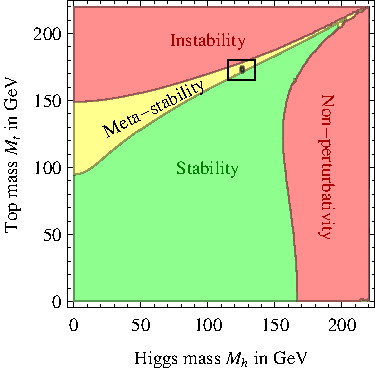
\includegraphics[width=.46 \linewidth]{figures/SMht}
 		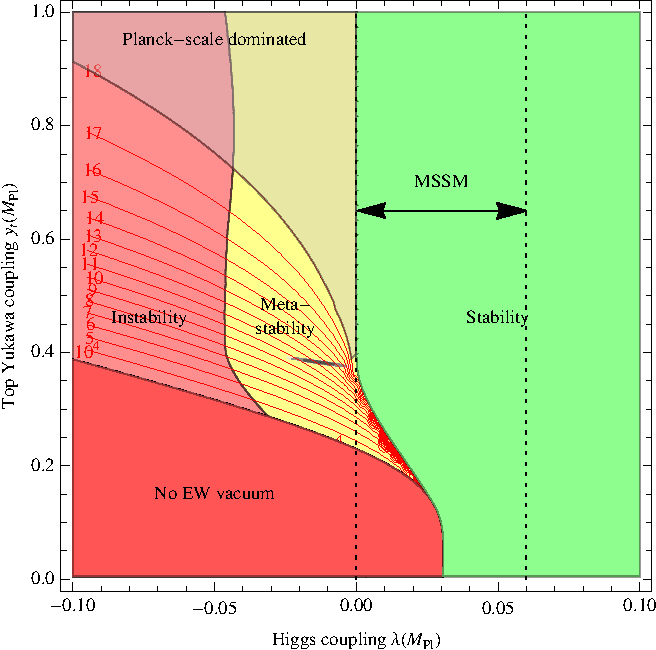
\includegraphics[width=.46 \linewidth]{figures/Ath}
 		\caption{.}
 		\label{fig:vacuum}
 	\end{center}
 \end{figure}
%%%%%% HERE
\section{Experimental measurements in the Higgs sector}
We also provide in this appendix the experimental measurements of the signal strengths at the LHC Run II and the CMS projections for the HL-LHC (scenario S2, see \cite{Cepeda:2019klc}) that we used in the fits in this paper. These inputs are summarised in table~\ref{table:resHiggsExp}.
\begin{figure}[t!]
	\begin{center}
		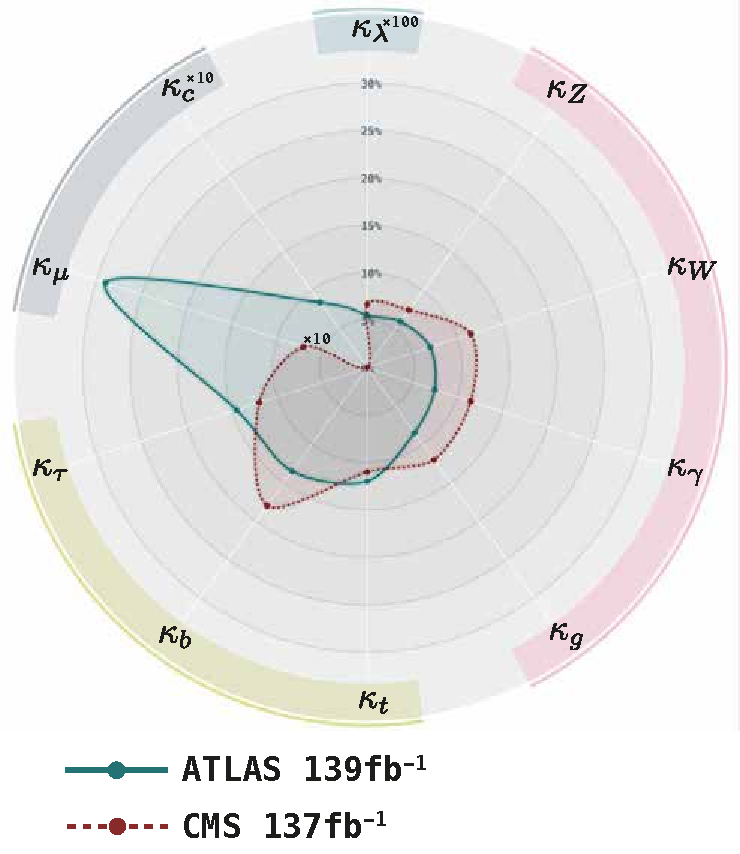
\includegraphics[width=8cm]{figures/kaappa_higgs}
		\caption{ff.\label{fig:higgs_kappa} }
	\end{center}
\end{figure}
\newpage
\begingroup
\thispagestyle{plain}
\begin{table}[htb!]
\centering
\vspace{-1 cm}
 \footnotesize{ 
	{\renewcommand{\arraystretch}{0.75 }%
\begin{tabular}{clccc}
\toprule
\toprule
\multirow{5}{*}{ {\normalsize Production}}  &\multirow{5}{*}{ {\normalsize Decay}}&\multicolumn{2}{c}{ $\mu_{\mathrm{Exp}} \pm \delta \mu_{\mathrm{Exp}}$  (symmetrised)} &\multirow{5}{*}{ {\normalsize Ref.}} \\
%\cmidrule(r){3-4}
&   & { \bf     \scriptsize           LHC Run-II}&{ \bf  \scriptsize HL-LHC}&   \\
\cmidrule(r){3-4}
&   & { \scriptsize                   CMS $137 \, \mathrm{fb}^{-1} $}&  \multirow{2}{*}{CMS $3 \, \mathrm{ab}^{-1}$}&   \\
&   &  { \CG \scriptsize                   ATLAS $139 \, \mathrm{fb}^{-1} $} & &  \\
\midrule
\midrule
\multirow{ 13}{*}{ \normalsize ggF}         & \multirow{2}{*}{$h\to \gamma  \gamma$} & { \scriptsize                  $0.99 \pm 0.12$}& \multirow{2}{*}{$1.000\pm 0.042$}& \multirow{2}{*}{\cite{ATLAS:2020qdt,CMS:2021kom,CMS-PAS-FTR-18-011}}\\
                                           &                                                          &{ \scriptsize                   \CG $1.030 \pm 0.110$}&& \\ 
                                           \cmidrule(r){2-5}
                                           %%%%%%
                                    &  \mr{$h\to Z Z^*$}          & { \scriptsize                  $0.985 \pm 0.115$}&\multirow{2}{*}{$1.000 \pm 0.040$}&\multirow{7}{*}{\cite{ATLAS:2020qdt,CMS:2020gsy,CMS-PAS-FTR-18-011}}  \\
                                     &                                                      &{ \scriptsize                   \CG $0.945 \pm 0.105$}&& \\
                                     \cmidrule(r){2-4}
                                       %%%%%%
                                    &\mr{ $h\to W W^*$}         & { \scriptsize                  $1.285 \pm 0.195$} &\mr{ $1.000 \pm 0.037$} &\\
                                    & &                                            { \scriptsize                   \CG$1.085 \pm 0.185$} & &\\
                                                                         \cmidrule(r){2-4}
                                     %%%%%%
                                    &\mr{ $h\to \tau^+\tau^- $ }         & { \scriptsize                  $0.385 \pm 0.385$} &\mr{ $1.000 \pm 0.055$} &\\
                                 & &                                            { \scriptsize                   \CG$1.045 \pm 0.575$} & &\\
                                 \cmidrule(r){2-5}
                                 %%%%%%

                                  &\mr{ $h\to  b \bar b$  }      & { \scriptsize                 $2.54 \pm 2.44$} &\mr{ $1.000 \pm 0.247$} &\mr{\cite{CMS:2020gsy,CMS-PAS-FTR-18-011}}\\
                               & &                                            { \scriptsize                   \CG--} & &\\
                                 \cmidrule(r){2-5}
                               %%%%%%  %%%%%%   %%%%%%
                                  &\mr{ $h\to  \mu^+ \mu^-$  }      & { \scriptsize      $0.315 \pm 1.815$} &\mr{ $1.000 \pm 0.138$} &\mr{\cite{CMS:2020gsy,CMS-PAS-FTR-18-011} }\\
& &                                            { \scriptsize                   \CG--} & &\\
%%%%%%  %%%%%%   %%%%%%                               
\midrule
\midrule
%\crowcolor
\multirow{13}{*}{ \normalsize VBF}      
                                     %%%%%%
										&\mr{ $h\to \gamma  \gamma$ }         & { \scriptsize                  $1.175 \pm 0.335$ } &\mr{ $1.000 \pm 0.128$} & \mr{\cite{ATLAS:2020qdt,CMS:2021kom,CMS-PAS-FTR-18-011}}\\
										& &                                           { \scriptsize                   \CG$1.325 \pm 0.245$} & &\\
\cmidrule(r){2-5}
%%%%%%                                   
                                     &\mr{$h\to Z Z^*$ }         & { \scriptsize                  $0.62 \pm 0.41$ } &\mr{ $1.000 \pm 0.134$} & \multirow{7}{*}{\cite{ATLAS:2020qdt,CMS:2020gsy,CMS-PAS-FTR-18-011}}\\
                                    & &                                            { \scriptsize                   \CG$1.295 \pm 0.455$} & &\\
                                                                                             \cmidrule(r){2-4}
%%%%%%

                                   &\mr{$h\to W W^*$}         & { \scriptsize                  $0.65 \pm 0.63$ } &\mr{ $1.000 \pm 0.073$} & \\
                                    & &                                            { \scriptsize                   \CG$0.61 \pm 0.35$} & &\\
 \cmidrule(r){2-4}
%%%%%%0
                                   &\mr{$h\to \tau^+\tau^- $}         & { \scriptsize                  $1.055 \pm 0.295$ } &\mr{ $1.000 \pm 0.044$} & \\
& &                                            { \scriptsize                   \CG$1.17 \pm 0.55$} & &\\
\cmidrule(r){2-5}
%%%%%%0                                    
                                    &\mr{$h\to  b \bar b$}         & { \scriptsize                   -- } &\mr{--} & \mr{\cite{ATLAS:2020qdt} }\\
                                    & &                                            { \scriptsize                   \CG$3.055 \pm 1.645$} & &\\
                                    
                                  \cmidrule(r){2-5}
 %%%%%%  %%%%%%   %%%%%%
 &\mr{ $h\to  \mu^+ \mu^-$  }      & { \scriptsize               $3.325 \pm 8.075$} &\mr{ $1.000 \pm 0.540$} &\mr{ \cite{CMS-PAS-FTR-18-011}}\\
 & &                                            { \scriptsize                   \CG--} & & \\                                   
\midrule
\midrule
\multirow{10}{*}{ \normalsize  $t\bar t h$} 
%%%%%%0                                    
&\mr{ $h\to \gamma  \gamma$}         & { \scriptsize                $1.43 \pm 0.30$ } &\mr{$1.000 \pm 0.094$} & \mr{ \cite{ATLAS:2020qdt,CMS:2021kom,CMS-PAS-FTR-18-011} }\\
& &                                            { \scriptsize                   \CG$0.915 \pm 0.255$} & &\\

\cmidrule(r){2-5}

                                    
%%%%%%0                                    
&\multirow{3}{*} { $h\to V V^*$   }         & { \scriptsize              $0.64 \pm 0.64$({\color{Mahogany}$ZZ^*$}) } &{ \scriptsize   $1.000 \pm 0.246$ ({\color{Mahogany}$ZZ^*$}) } & \multirow{8}{*}{\cite{ATLAS:2020qdt,CMS:2020gsy,CMS-PAS-FTR-18-011}}  \\
& &                                            { \scriptsize                   $0.945\pm 0.465$ ({\color{Mahogany} $W W^*$})} & { \scriptsize   $1.000 \pm 0.097$ ({\color{Mahogany} $W W^*$})} &\\
& &                                            { \scriptsize                   \CG $1.735 \pm 0.545$} & { \scriptsize   --}&\\
\cmidrule(r){2-4}                                    

&\mr{$h\to \tau^+\tau^- $}         & { \scriptsize                $0.845 \pm 0.705$} &\mr{ $1.000 \pm 0.149$} & \\
& &                                            { \scriptsize                   \CG $1.27 \pm 1.0$} & &\\
\cmidrule(r){2-4}                                    

&\mr{ $h\to  b \bar b$  }         & { \scriptsize                 $1.145 \pm 0.315$} &\mr{ $1.000 \pm 0.116$} & \\
& &                                            { \scriptsize                   \CG $0.795 \pm 0.595$} & &\\                                                        
\midrule
\midrule
\multirow{9}{*}{ \normalsize $Vh$}        

                      
&\mr{ $h\to \gamma  \gamma$  }         & { \scriptsize   $0.725 \pm 0.295$ } &{ \scriptsize   $1.000 \pm 0.233$ ({\color{Mahogany}$Zh$}) } & \multirow{2}{*}{ \cite{ATLAS:2020qdt,CMS:2021kom,CMS-PAS-FTR-18-011}  }  \\
& &                                            { \scriptsize                   \CG $1.335 \pm 0.315$} & { \scriptsize   $1.000 \pm 0.139$ ({\color{Mahogany} $W^\pm h$})} &\\
\cmidrule(r){2-5}           
%%%%%%0              
                                    
&\mr{ $h\to Z Z^*$    }         & { \scriptsize   $1.21 \pm 0.85$ } &{ \scriptsize   $1.000 \pm 0.786$ ({\color{Mahogany}$Zh$}) } & \multirow{2}{*}{ \cite{ATLAS:2020qdt,CMS:2020gsy,CMS-PAS-FTR-18-011}  }  \\
& &                                            { \scriptsize                   \CG $1.635 \pm 1.025$} & { \scriptsize   $1.000 \pm 0.478$ ({\color{Mahogany} $W^\pm h$})} &\\
\cmidrule(r){2-5}           
%%%%%%0                                         
                                  
 &\mr{ $h\to W W^*$    }         & { \scriptsize   $1.850\pm 0.438$ } &{ \scriptsize   $1.000 \pm 0.184$ ({\color{Mahogany}$Zh$}) } & \multirow{2}{*}{  \cite{CMS:2021ixs,CMS-PAS-FTR-18-011} }  \\
 & &                                            { \scriptsize                   \CG --} & { \scriptsize   $1.000 \pm 0.138$ ({\color{Mahogany} $W^\pm h$})} &\\
 \cmidrule(r){2-5}           
 %%%%%%0                                                                                                            
 &\mr{$h\to  b \bar b$      }         & { \scriptsize  -- } &{ \scriptsize   $1.000 \pm 0.065$ ({\color{Mahogany}$Zh$}) } & \multirow{2}{*}{  \cite{ATLAS:2020qdt,CMS-PAS-FTR-18-011} }  \\
& &                                            { \scriptsize                   \CG $1.025 \pm 0.175$} & { \scriptsize   $1.000 \pm 0.094$ ({\color{Mahogany} $W^\pm h$})} &\\

%%%%%%0                                        
                                    
\midrule
\midrule
\multirow{2}{*}{ \normalsize $Zh$ { \scriptsize {\color{Mahogany} CMS     }   }}    & $h\to \tau^+\tau^- $ & $1.645 \pm 1.485$&\multirow{5}{*}{--} &\multirow{5}{*}{ \cite{CMS:2020gsy} }  \\
& $h\to  b \bar b$       &$0.94 \pm 0.32$&&\\                         
 \cmidrule(r){2-3}    
\multirow{2}{*}{ \normalsize $W^\pm h${ \scriptsize {\color{Mahogany} CMS     }   }}           & $h\to \tau^+\tau^- $ &$3.08 \pm 1.58$&&\\
& $h\to  b \bar b$      & $1.28 \pm 0.41$&&\\                  
\midrule
\midrule
\end{tabular}
}
}
\caption{The experimental single Higgs production and decay rates measurements from the  complete  data of LHC Run II and projections for the HL-LHC. The uncertainties were symmetrised here. The table is published in~\cite{Alasfar:2022zyr}.  }
\label{table:resHiggsExp}
\end{table} 
\endgroup